
\chapter{Medicínska podstata problému} \label{kap:Motivacia}

\pagestyle{fancy}
\fancyhf{}
\fancyfoot[CE,CO]{\thepage}
%\renewcommand{\footrulewidth}{1pt}
\lhead{Medicínska podstata problému}

Spánkové poruchy postihujú približne 30% svetovej populácie. Podľa súčasnej platnej
medzinárodnej klasifikácie spánkových porúch sú respiračné spánkové poruchy druhým
najčastejšie sa vyskytujúcim ochorením /cite{neviem}

Respiračné spánkové apnoické ochorenia delíme na:
obštrukčné (OSAS): dospelí pacienti, pediatrickí pacienti
centrálne (CSA): Cheine-Stokes dýchanie, Primárne, ...
zmiešané: kombinované CSA a OSAS

Syndróm obštrukčného spánkového apnoe (OSAS) je respiračná choroba, ktorá spôsobuje
prerušenie oronazálnej ventilácie pri pretrvávajúcom dychovom úsilí na aspoň 10 sekúnd a
opakuje sa viac ako 5 krát za hodinu (2). Na jej vzniku sa vo významnej miere podieľa znížená
priechodnosť horných dýchacích ciest a zmena mechanizmu mäkkých štruktúr horných dýchacích
ciest. Najvýznamnejším rizikovým faktorom vzniku OSAS je anatomické zúženie horných
dýchacích ciest spôsobené predovšetkým: obezitou, kraniofaciálnymi abnormalitami, hypopláziou
tváre, zväčšeným objemom mäkkých tkanív, hypertrofiou tonzíl, zväčšením uvuly a dĺžky
mäkkého podnebia (3).

K presnému stanoveniu OSAS diagnózy sa vykonáva špeciálne komplexné vyšetrenie nazývané
polysomnografia (PSG). Ide o celonočné monitorovanie pacienta pomocou snímačov a senzorov,
ktoré dávajú lekárovi informáciu o dýchaní, ronchopátii, činnosti srdca, charaktere spánku a jeho
jednotlivých cykloch, o polohe tela a o okysličovaní organizmu. PSG sa vykonáva v
akreditovanom spánkovom laboratóriu, ktoré musí byť vybavené potrebnou meracou technikou. Z
výsledkov sa následne určuje konkrétny spôsob liečby (4).

PSG je považovaná za štandard pre diagnostiku OSAS, avšak toto vyšetrenie je finančne
nákladné a časovo náročné. Navyše na Slovensku ale aj vo svete je problém s nedostatkom
spánkových laboratórií, čo spôsobuje dlhé čakacie doby.

Kvôli zníženiu potreby používania PSG adolescentnou skupinou pacientov bol vytvorený
validovaný dotazník nazývaný Klinický záznam o spánku (SCR). Ten pomocou kombinácie
informácií z klinického vyšetrenia, skúmania subjektívnych symptómov pacienta a skúmania
prítomnosti ADHD dokáže s určitou presnosťou identifikovať prítomnosť OSAS. Pozitívni
pacienti sú následne uprednostňovaní na vyšetrenie PSG (5).

Vyšetrenie pomocou kontaktných meracích prístrojov je pre pediatrických pacientov často krát
stresujúce. Deti sú nepokojné a nedokážu spolupracovať s doktorom, čo predlžuje vyšetrenie a
vnáša chybu merania do dotazníka. Z toho dôvodu je požiadavka na vytvorenie meracieho
systému, ktorý by dokázal zmerať požadované parametre bezkontaktne.

Alternatívnym riešením je vytvorenie skenovacieho zariadenia, ktoré dokáže s určitou
precíznosťou geometricky aj textúrovo reprodukovať pacienta v 3D formáte. Následné meranie
na existujúcom modeli je možné vykonávať bez prítomnosti pacienta, taktiež je možné ho
opakovať alebo dodatočne zmerať aj iné tvárové parametre. Pri softvérovom meraní tvárových
parametrov vzniká možnosť automatizácie.

\section{Aktuálny výskum v oblasti OSAS diagnostiky}

https://arxiv.org/pdf/1911.05628.pdf
\newpage
\subsection{Diagnostika pediatrickej OSA prostredníctvom klasifikácie tváre s použitím CNN}

V článku "Diagnosis of Pediatric Obstructive Sleep Apnea via FaceClassification with Persistent Homology and ConvolutionalNeural Networks" je opísaná štúdia, v ktorej sa snažia vytvoriť klasifikátor pre rozdelenie vysoko rizikových pacientov od tých menej rizikových. K analýze využívali 3D modely a 2D fotografie obsahujúce snímky 3D objektov. Podľa súčasných štúdií, na ktoré sa v práci odkazujú, využili pre klasifikáciu perzistentnú homológiu (PH) a konvolučné neurónové siete. Pri prvom prístupe analyzujú trojuholníkové siete cez geometrické príznaky tváre, pri CNN sa pre trénovanie používajú klasifikované 2D obrazy tváre. Použitý dátový set obsahoval 172 detských pacientov. Objekty boli  klasifikované do vyššej alebo nižšej rizikovej skupiny OSA lekárom. Každý 3D model podstúpil filtráciu (vyplnenie dier v sieti, vyhladenie) pri ktorej sa ale dbalo na to, aby nebola znehodnotená geometrická informácia. 

Z výsledkov PH vyplýva, že súčasné topologické analýzy dát neviedli k presnej klasifikácii. Niektoré rysy tváre síce môžu súvisieť s vysokým rizikom OSA, ale neboli postačujúce pre identifikáciu rizikových pacientov. 


\begin{figure}[h]
	\centering
	\begin{subfigure}[b]{0.32\textwidth}
		\centering
		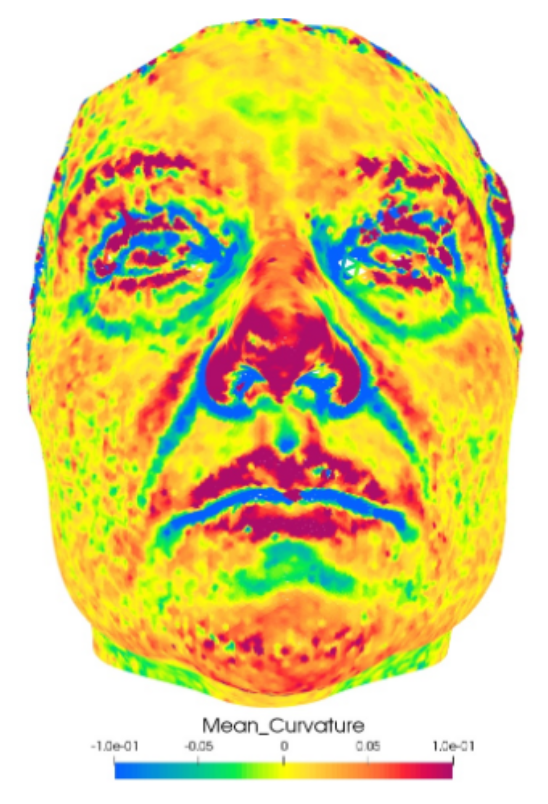
\includegraphics[width=0.95\textwidth]{figures/resers_a.png}
		\caption{}
		\label{fig:resers:a}
	\end{subfigure}
	\hfill
	\begin{subfigure}[b]{0.32\textwidth}
		\centering
		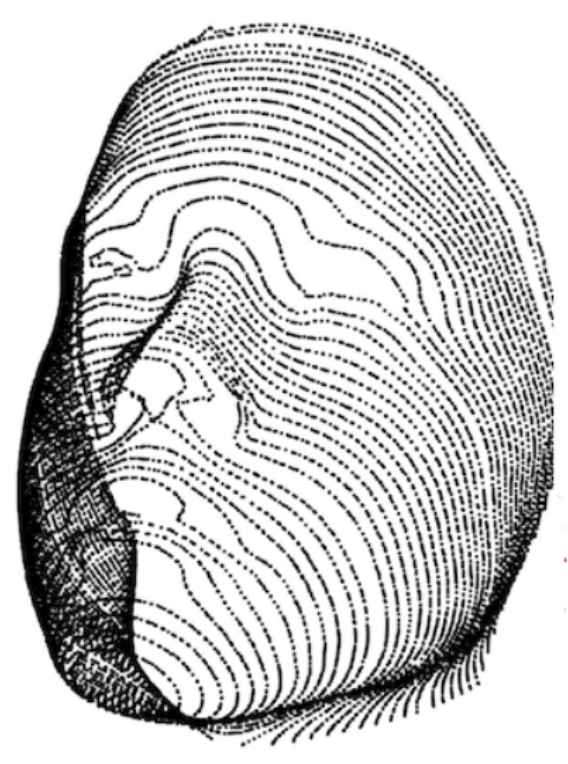
\includegraphics[width=\textwidth]{figures/resers_b.png}
		\caption{}
		\label{fig:resers:b}
	\end{subfigure}
	\hfill
	\begin{subfigure}[b]{0.32\textwidth}
		\centering
		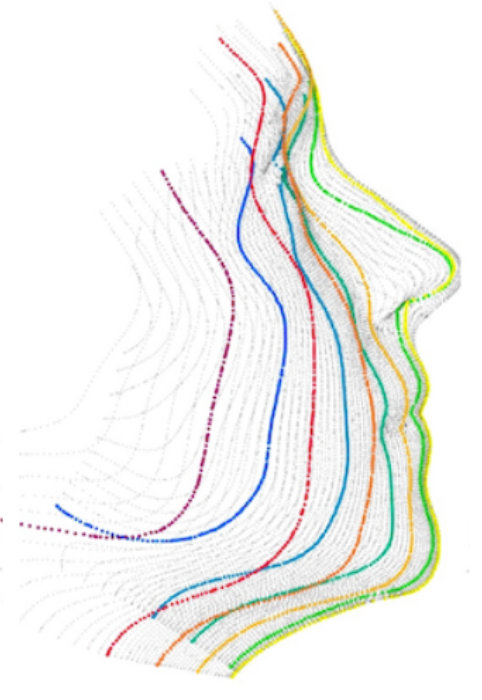
\includegraphics[width=0.95\textwidth]{figures/resers_c.png}
		\caption{}
		\label{fig:resers:c}
	\end{subfigure}
	\caption{Vstupné dáta pre PH klasifikáciu: (\textbf{a}) Priemerné hodnoty zakrivenia pre každý bod v mračne bodov. 
	(\textbf{b}) Krivky tváre
	(\textbf{c}) Geodetika medzi dvoma pacientmi. }
	\label{fig:resers}
\end{figure}

\newpage


Pre použitie CNN metódy boli z filtrovaných modelov vytvorené série snímok, ktoré zachytávali objekty z rôznych perspektív. Je to kvôli tomu, aby konvolučná neurónová sieť dokázala lepšie pochopiť povrch tváre. Následne boli dáta rozdelené v pomere $80\%$ pre trénovanie a $20\%$ pre testovanie. V článku sa používali CNN architektúry: InceptionV3, InceptionResV2, MobileNetV2 a NASNetLarge. Tie boli predtrénované na ImageNet datasete. 

Výsledky trénovania pre MobileNetV2 a NASNetLarge sú zobrazené na obr. \ref{fig:resers:d}. Z nich vyplýva, že validácia výstupného modelu nedosahovala očakávané výsledky. 


\begin{figure}[h]
	\centering
	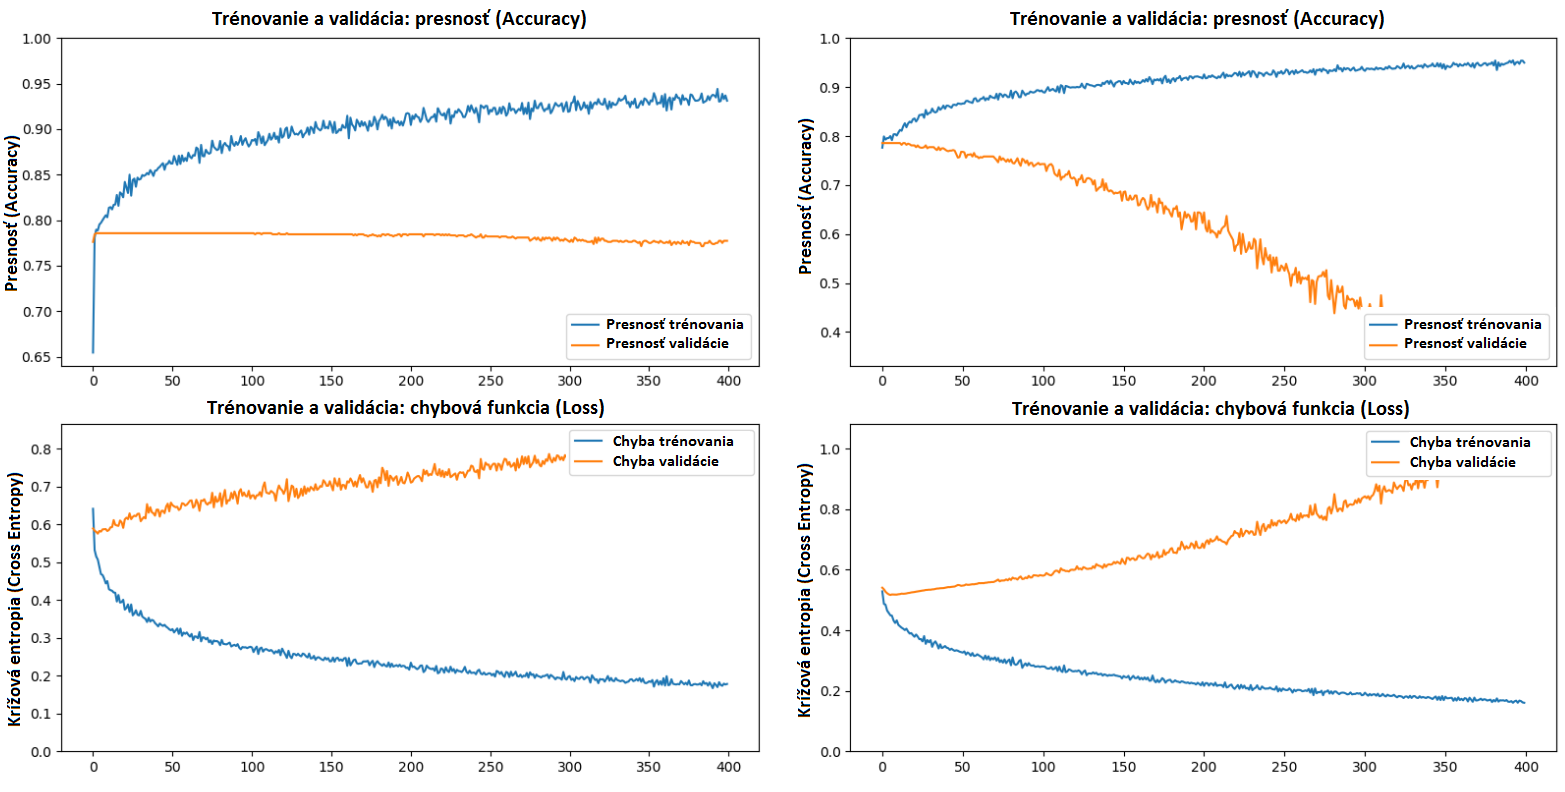
\includegraphics[width=\textwidth]{figures/resers_d.png}
	\caption{Kontinuálna impulzná modulácia TOF senzora}
	\label{fig:resers:d}
\end{figure}


\begin{table}[H]
	\caption{\label{tab:final_comp} Výsledky validácie pretrénovaných modelov pre použité CNN architektúry. }
	\centering
	\begin{tabular}{cccc}
		\toprule
		\textbf{InceptionV3} & \textbf{InceptionResV2} & \textbf{MobileNetV2} & \textbf{NASNetLarge}     \\ 
		\midrule
		\textbf{InceptionV3}           & ImageNet     	& TensorFlow    & $70 \pm 4$		\\ 
		\textbf{InceptionResV2}        & ImageNet		& TensorFlow  	& $71 \pm 5$		\\ 
		\textbf{MobileNetV2}           & ImageNet     	& TensorFlow    & $64 \pm 5$		\\ 
		\textbf{NASNetLarge}           & ImageNet     	& TensorFlow    & $72 \pm 2$		\\ 
		\bottomrule
	\end{tabular}
\end{table}

Možným dôvodom je, že dátové sety pediatrických OSA pacientov obsahujú malé množstvo klasifikovaných objektov. Ak by sa v budúcnosti vytvorila databáza, ktorá bude zhromažďovať potrebné dáta, je veľký predpoklad na zlepšenie presnosti klasifikovania OSA pacientov pomocou CNN.


\subsection{Predikcia OSA pomocou hlbokého učenia s použitím hĺbkovej mapy tváre}

V článku "Deep Learning of Facial Depth Maps for Obstructive Sleep Apnea Prediction" autori používajú pre detekciu OSA hĺbkové mapy a konvolučné neurónové siete. V teoretickom úvode sa odkazujú na súčasné trendy pri diagnostike OSA. Uvádzajú, že nové diagnostické metódy smerujú k využívaniu obrazovej informácii hlavy a krku pacienta. V ich práci sa zamerali na využitie hĺbkových máp, ktoré poskytovali informáciu o geometrických parametroch tváre a krku. 

3D dáta boli získané od pacientov, ktorí podstúpili PSG diagnostiku. Databáza bola tvorená z 39 mužských a 30 ženských skenov, ktoré boli vytvorené snímačom Arctec Eva. Tie boli následne filtrované, čím sa odstránili neželané artefakty. Z takto upravených modelov boli následne vytvorené 2D hĺbkové mapy.  

\begin{figure}[h]
	\centering
	\begin{subfigure}[b]{0.62\textwidth}
		\centering
		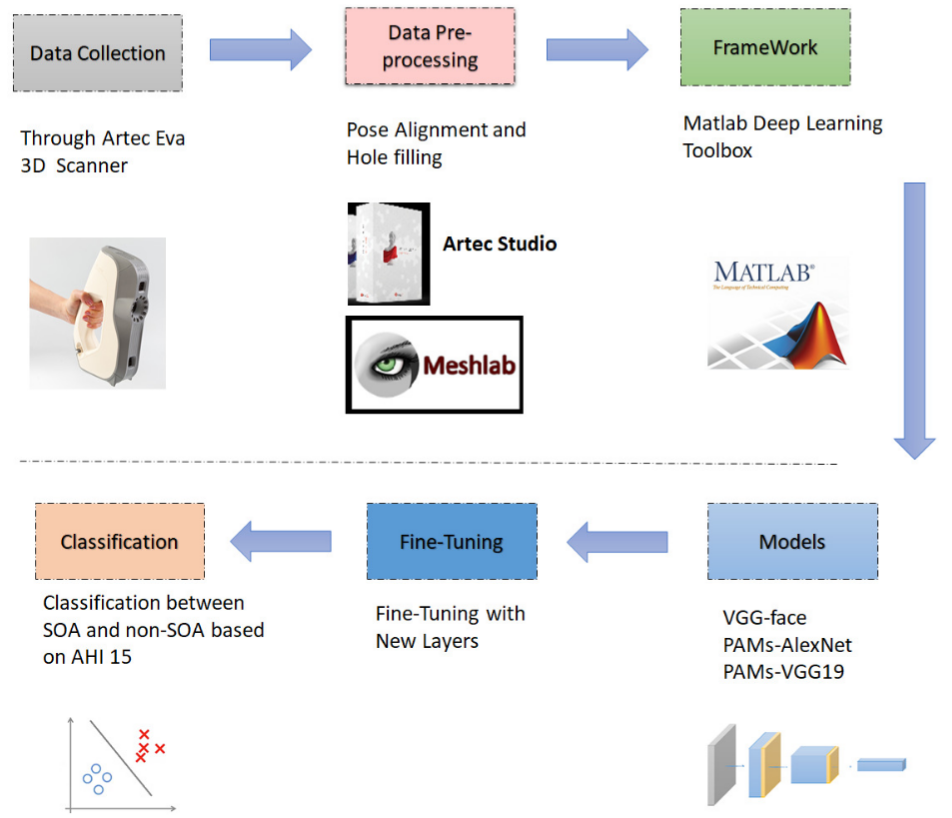
\includegraphics[width=\textwidth]{figures/resers_e.png}
		\caption{}
		\label{fig:resers:a}
	\end{subfigure}
	\hfill
	\begin{subfigure}[b]{0.37\textwidth}
		\centering
		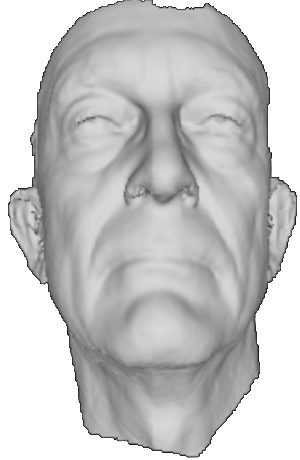
\includegraphics[width=\textwidth]{figures/resers_f.png}
		\caption{blablalblalblalasasas}
		\label{fig:resers:b}
	\end{subfigure}
	\caption{Vstupné dáta pre PH klasifikáciu: (\textbf{a}) Priemerné hodnoty zakrivenia pre každý bod v mračne bodov. 
	(\textbf{b}) Krivky tváre
	(\textbf{c}) Geodetika medzi dvoma pacientmi. }
\label{fig:resers}
\end{figure}

K trénovaniu si vybrali tri rozdielne neuronové siete, ktoré už boli pretrénované pre detekciu a rozpoznanie tváre. Neboli však trénované na hĺbkových mapách.  VCG-Face bol trénovaný na 2.6 miliónovom datasete s presnosťou 98.95\%. Taktiež boli použití Pose-Aware CNN modely AlexNet a VGG-19. 

Pre jemné dolaďovanie modelov bol použitý \textit{Matlab deep learning toolbox}. Z databázy hĺbkových máp bolo 70\% použitých pre trénovanie a 30\% pre validáciu. 

\begin{table}[H]
	\caption{\label{tab:final_comp} Presnosť klasifikácie použitých modelov. }
	\centering
	\begin{tabular}{cccc}
		\toprule
		\textbf{InceptionV3} & \textbf{InceptionResV2} & \textbf{MobileNetV2} & \textbf{NASNetLarge}     \\ 
		\midrule
		\textbf{InceptionV3}           & ImageNet     	& TensorFlow    & $70 \pm 4$		\\ 
		\textbf{InceptionResV2}        & ImageNet		& TensorFlow  	& $71 \pm 5$		\\ 
		\textbf{MobileNetV2}           & ImageNet     	& TensorFlow    & $64 \pm 5$		\\ 
		\textbf{NASNetLarge}           & ImageNet     	& TensorFlow    & $72 \pm 2$		\\ 
		\bottomrule
	\end{tabular}
	\end{table